\documentclass[12pt,letterpaper]{article}
\usepackage[utf8]{inputenc}
\usepackage[spanish]{babel}
\usepackage{graphicx}
\usepackage[left=2cm,right=2cm,top=2cm,bottom=2cm]{geometry}
\usepackage{graphicx} % figuras
% \usepackage{subfigure} % subfiguras
\usepackage{float} % para usar [H]
\usepackage{amsmath}
%\usepackage{txfonts}
\usepackage{stackrel} 
\usepackage{multirow}
\usepackage{enumerate} % enumerados
\renewcommand{\labelitemi}{$-$}
\renewcommand{\labelitemii}{$\cdot$}
% \author{}
% \title{Caratula}
\begin{document}

% Fancy Header and Footer
% \usepackage{fancyhdr}
% \pagestyle{fancy}
% \cfoot{}
% \rfoot{\thepage}
%

% \usepackage[hidelinks]{hyperref} % CREA HYPERVINCULOS EN INDICE

% \author{}
\title{Caratula}

\begin{titlepage}
\begin{center}
\large{UNIVERSIDAD PRIVADA-DE-TACNA}\\
\vspace*{-0.025in}
\begin{figure}[htb]
\begin{center}

\includegraphics[width=8cm]{./Imagenes/logo}
\end{center}
\end{figure}
\vspace*{0.15in}
INGENIERIA DE SISTEMAS  \\

\vspace*{0.5in}
\begin{large}
TITULO:\\
\end{large}

\vspace*{0.1in}
\begin{Large}
\textbf{INFORME DE LABORATORIO No 04} \\
\end{Large}

\vspace*{0.3in}
\begin{Large}
\textbf{CURSO:} \\
\end{Large}

\vspace*{0.1in}
\begin{large}
BASE DE DATOS II\\
\end{large}

\vspace*{0.3in}
\begin{Large}
\textbf{DOCENTE(ING):} \\
\end{Large}

\vspace*{0.1in}
\begin{large}
 Patrick Cuadros Quiroga\\
\end{large}

\vspace*{0.2in}
\vspace*{0.1in}
\begin{large}
Integrantes: \\
\begin{flushleft}
Acosta Ortiz, Orlando Antonio                  \hfill	(2015052775) \\
Ramirez Ticona, Orestes                           \hfill  (2015053236) \\
Zegarra Reyes, Roberto  		            \hfill 	(2010036175) \\
Catari Cabrera, Yofer Nain 		\hfill 	(2017059289) \\
Mamani Maquera, Jorge Luis                   \hfill 	(2016055236) \\
Rivas Rios, Marko Antonio                       \hfill 	(2016054461) \\
\end{flushleft}
\end{large}
\end{center}

\end{titlepage}


\tableofcontents % INDICE
\thispagestyle{empty} % INDICE SIN NUMERO
\newpage
\setcounter{page}{1} % REINICIAR CONTADOR DE PAGINAS DESPUES DEL INDICE

\section{Informacion General} 

\begin{itemize}
\subsection{Objetivos:}
	\item Conocer los fundamentos sobre contenedores y Docker.
	\item Poder instalar correctamente una instancia.
\subsection{Equipos, materiales, programas y recursos utilizados:}
	\item Virtualización activada en el BIOS.
	\item Windows 10 64bit: Pro, Enterprise o Education, con al menos 4GB de RAM.
	\item Docker Desktop
	\item Microsoft SQL Server 2017 o superior

\end{itemize}

\section{Marco Teorico} 

\begin{itemize}
\subsection{ Docker:}
	\item Tener un docker que provea el gestor de base de datos es muy útil porque se reducen tiempos de instalación y configuración y en caso de tener un error muy grave en la configuración es tan sencillo resolverlo como borrar el contenedor y crear uno nuevo.
          \item Los contenedores funcionan bien para desarrollo y tal vez algunos ambientes de evaluación para el cliente, pero para ambientes productivos para nada se recomiendan, en estos casos siempre será lo mejor que se cuente con una base de datos instalada en el servidor.
         \item Sirven para desplegar aplicaciones en un entorno virtual aislado, pero sin el overhead de tener un Sistema Operativo (SO) nuevo como se tiene en una Virtual Machine (VM).

\subsection{Oracle Database en Docker:}
	\item Los productos de Oracle son compatibles con Docker si el sistema operativo del host es Oracle Linux 7, pero no necesita usar un host OL7 para que esto funcione. Puedes ver cómo instalar Docker en OL7 .
	\item Usar imágenes de Oracle Container Registry o de Docker Store tiene la ventaja que los binarios de instalación vienen incluidos, lo que no es permitido por licencia en el resto de las distribuciones. 


\end{itemize}








\section{Procedimientos} 

\begin{itemize}
\subsection{ Iniciando Docker}


	\item Abrir el menu inicio y buscar la aplicación Docker for Windows.
		\begin{figure}[H]
		\begin{center}
		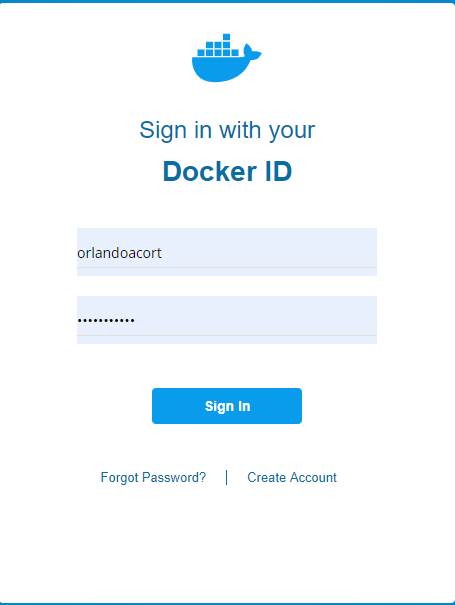
\includegraphics[width=8cm]{./Imagenes/2}
		\end{center}
		\end{figure}

	\item Ubicar la aplicación PowerShell, ejecutarla como Administrador. En la ventana de comandos de PowerShell escribir
lo siguiente.
		\begin{figure}[H]
		\begin{center}
		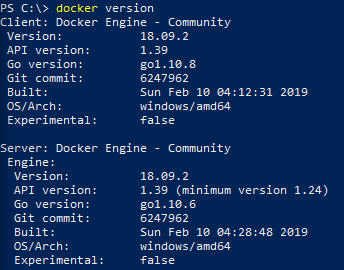
\includegraphics[width=8cm]{./Imagenes/1}
		\end{center}
		\end{figure}
     
\subsection{ Creando un contenedor con Oracle Database para Linux}
	\item En un navegador de internet acceder a la dirección https://hub.docker.com/. Iniciar sesión o crear una cuenta nueva
	\item Buscar el repositorio para Oracle Database. Ingresar y proceder con el CheckOut, completar los datos y aceptar las condiciones obligatorias para obtener el acceso al contenido.
		\begin{figure}[H]
		\begin{center}
		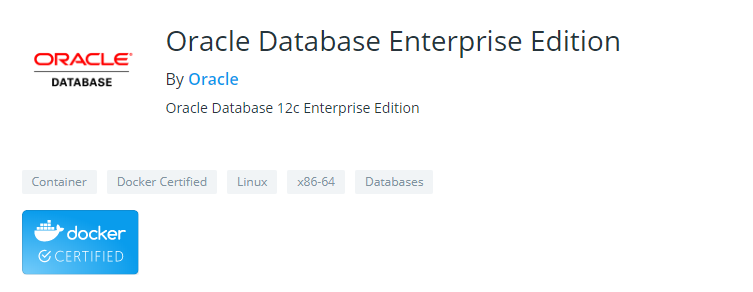
\includegraphics[width=8cm]{./Imagenes/3}
		\end{center}
		\end{figure}
	\item En la ventana de PowerShell, escribir el siguiente comando:
		\begin{figure}[H]
		\begin{center}
		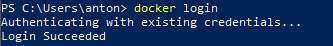
\includegraphics[width=9cm]{./Imagenes/4}
		\end{center}
		\end{figure}
	\item Ejecutar el siguiente comando en Powershell, lo cual descargará la imagen del contenedor de Oracle Database en un servidor Linux
		\begin{figure}[H]
		\begin{center}
		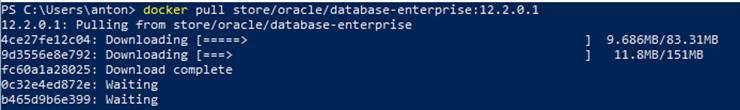
\includegraphics[width=15cm]{./Imagenes/5}
		\end{center}
		\end{figure}
	\item Seguidamente ejecutar el comando, como respuesta se visualizará un ID que corresponde al contenedor.
		\begin{figure}[H]
		\begin{center}
		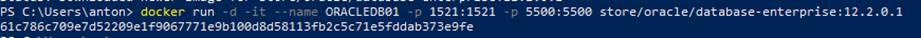
\includegraphics[width=15cm]{./Imagenes/6}
		\end{center}
		\end{figure}
	\item Verificar que el contenedor se esté ejecutando correctamente mediante el comando:
		\begin{figure}[H]
		\begin{center}
		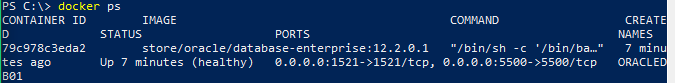
\includegraphics[width=15cm]{./Imagenes/7}
		\end{center}
		\end{figure}
	\item Cuando el estado del contenedor sea “healthy”, en la consola de Powershell, ejecutar el siguiente comando:
		\begin{figure}[H]
		\begin{center}
		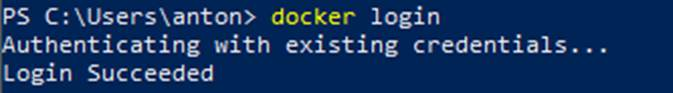
\includegraphics[width=15cm]{./Imagenes/8}
		\end{center}
		\end{figure}
	\item En la línea de comentados de SQL*Plus, escribir lo siguiente
		\begin{figure}[H]
		\begin{center}
		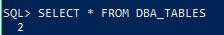
\includegraphics[width=8cm]{./Imagenes/9}
		\end{center}
		\end{figure}
	\item Escribir el comando quit para cerrar la sesión de SQL*Plus
		\begin{figure}[H]
		\begin{center}
		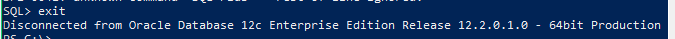
\includegraphics[width=15cm]{./Imagenes/10}
		\end{center}
		\end{figure}
	\item En una pestaña nueva del navegador de internet acceder a la siguiente dirección:https://localhost:5500/em. Iniciar sesión con los siguientes datos:
		\begin{figure}[H]
		\begin{center}
		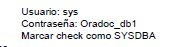
\includegraphics[width=4cm]{./Imagenes/t1}
		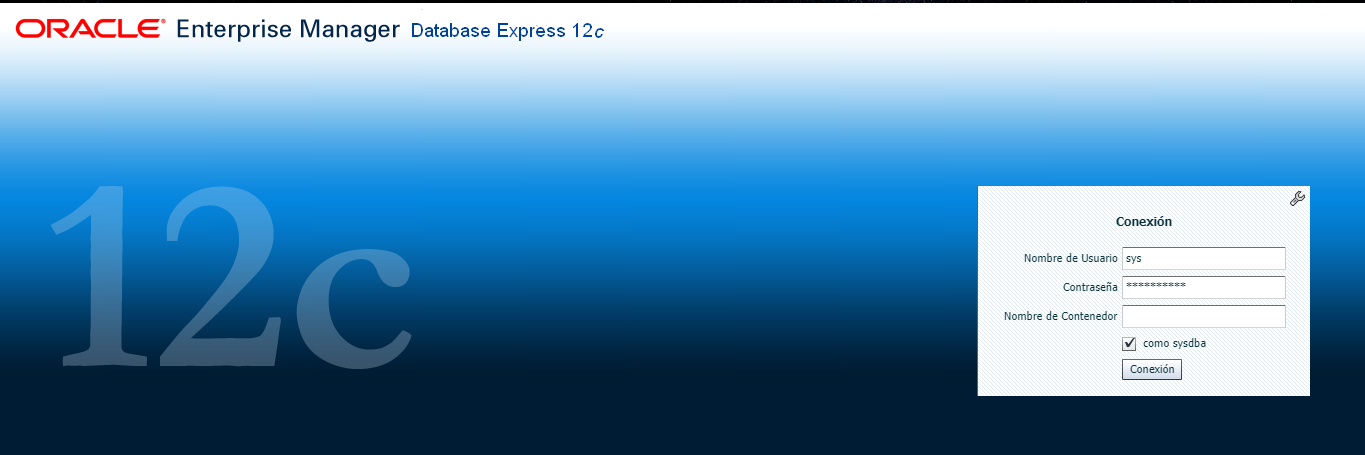
\includegraphics[width=15cm]{./Imagenes/11}
		\end{center}
		\end{figure}
	\item Luego se visualizará la siguiente ventana. Cerrar sesión y la pestaña del navegador de internet.
		\begin{figure}[H]
		\begin{center}
		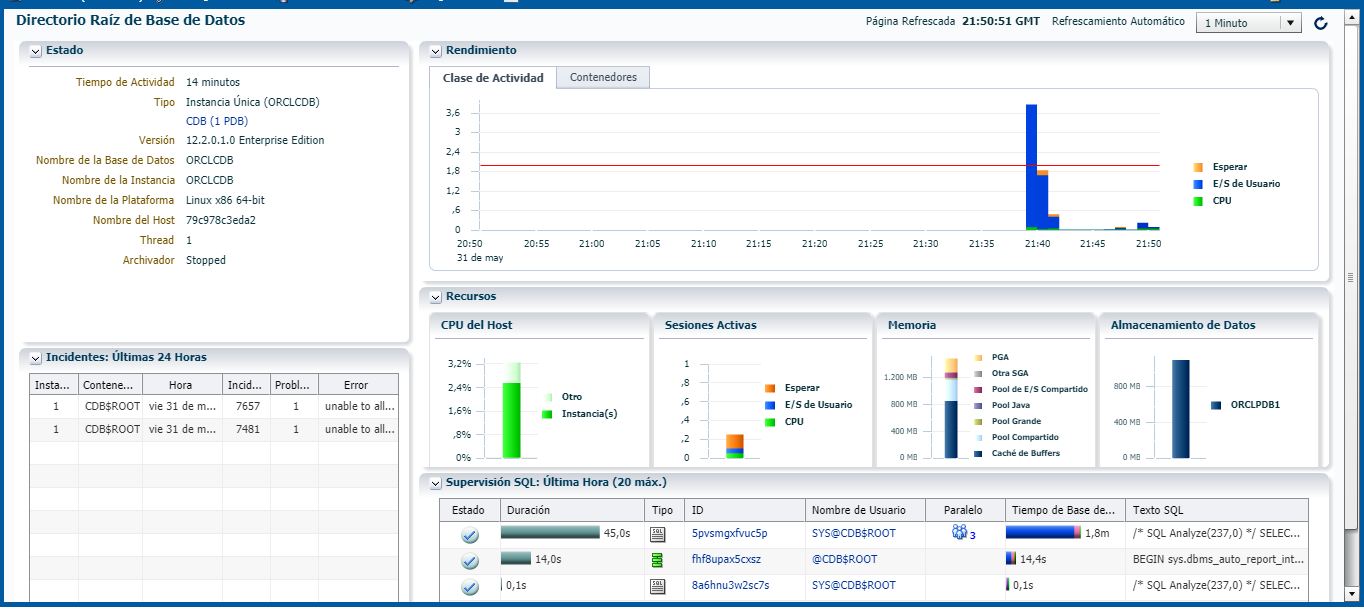
\includegraphics[width=15cm]{./Imagenes/12}
		\end{center}
		\end{figure}
	\item Iniciar el aplicativo Oracle SQL Developer, crear una nueva conexión con los siguientes parámetros:
		\begin{figure}[H]
		\begin{center}
		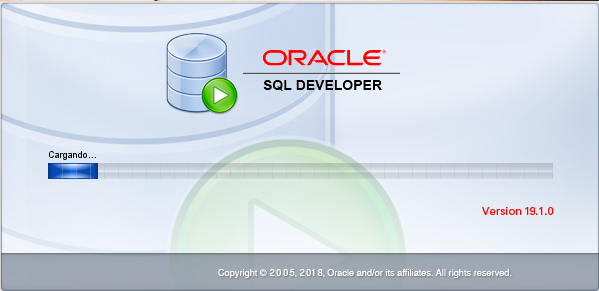
\includegraphics[width=15cm]{./Imagenes/131}
		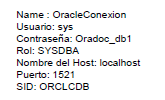
\includegraphics[width=5cm]{./Imagenes/t2}
		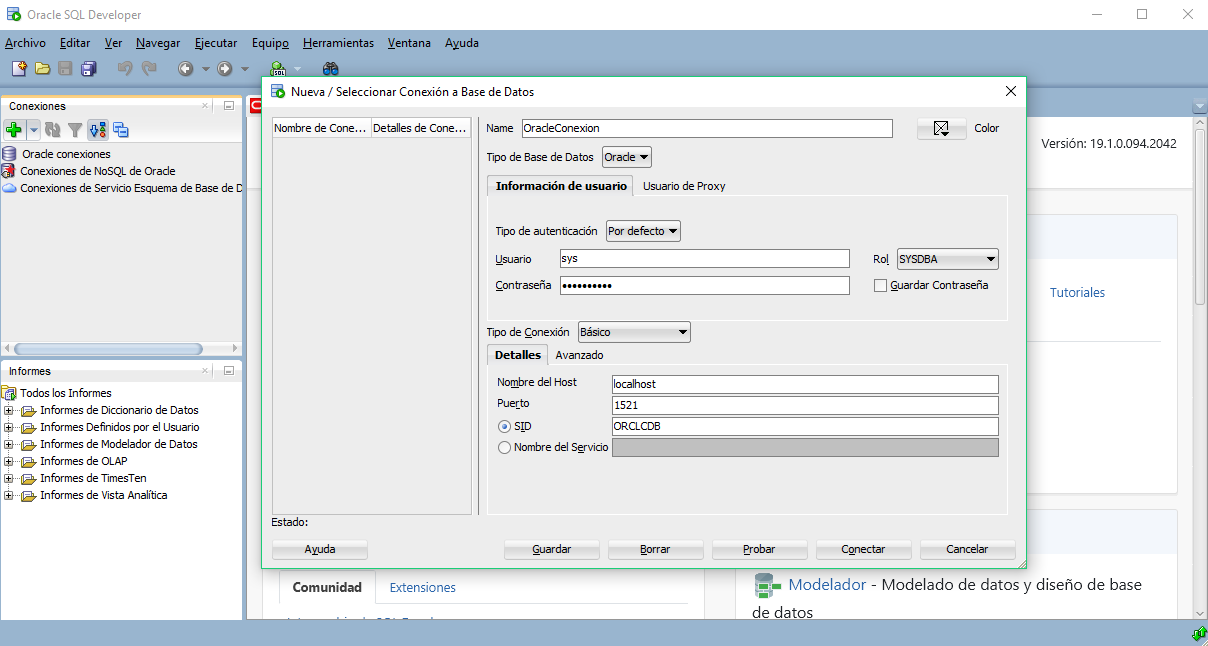
\includegraphics[width=15cm]{./Imagenes/13}
		\end{center}
		\end{figure}
	\item Iniciar una nueva consulta, escribir y ejecutar lo siguiente; deberá retornar varios registros que representan las tablas de las base de datos
		\begin{figure}[H]
		\begin{center}
		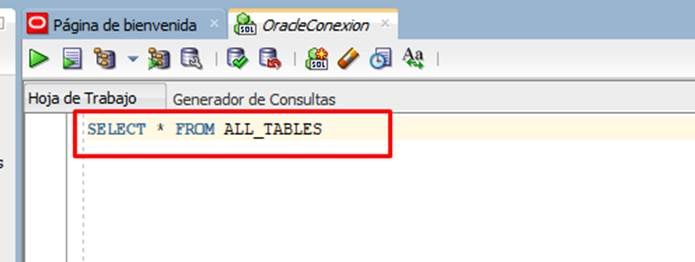
\includegraphics[width=15cm]{./Imagenes/141}
		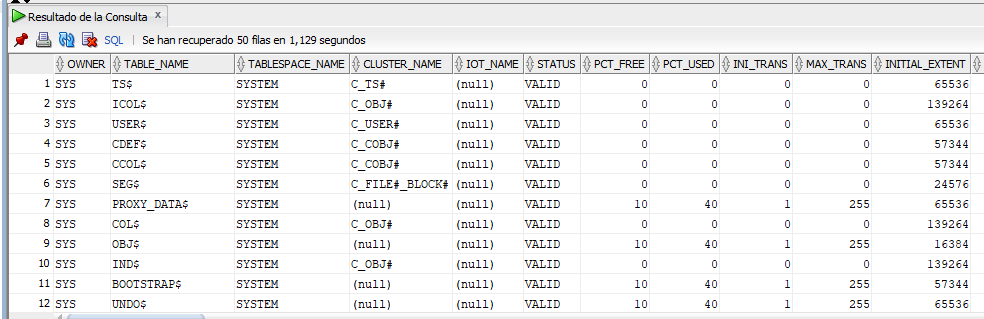
\includegraphics[width=15cm]{./Imagenes/14}
		\end{center}
		\end{figure}
	\item Cerrar la aplicación Oracle SQL Developer
	\item En PowerShell ejecutar el siguiente comando. Y verificar la eliminación del contenedor con ejecutando
		\begin{figure}[H]
		\begin{center}
		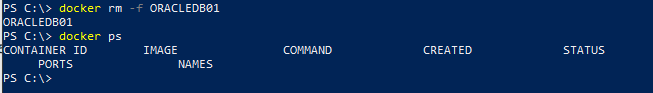
\includegraphics[width=12cm]{./Imagenes/15}
		\end{center}
		\end{figure}


       
\end{itemize}
		
\section{Analisis  de Resultados} 


\subsection{Actividades Encargadas}
	\begin{itemize}
		\item 1. ¿Con qué comando(s) puedo iniciar y detener una instancia de Oracle, detalle cada uno de los pasos y opciones,
		utilizando Docker?
		
		\item2. ¿Con qué comando(s) puedo iniciar y detener el Listener y el Enterprise manager, detalle cada uno de los pasos y
		opciones, utilizando Docker?
		\item 3. Genere un nuevo contenedor y cree un espacio de tablas con las siguientes características.
		Nombre : FINANCIERA:
		• DATOS (dbf) : Tamaño Inicial : 50MB, Incremento: 10MB, Ilimitado
		• INDICES (dbf) Tamaño Inicial : 100MB, Incremento: 20MB, Maximo: 1GB
		• HISTORICO (dbf) Tamaño Inicial : 100MB, Incremento: 50MB, Ilimitado
		¿Cuál sería el script SQL que generaría esta base de datos?
		\item
	\end{itemize}









\section{Conclusiones}
\begin{itemize}
	\item Docker resulta util ya que de amanera muy sencilla se puede disponer de diferentes gestores de Base de Datos.
	
	\item Resulta muy  factible tener varias bases de datos disponibles o además que existieran y comparen diferentes versiones de bases de datos a la vez.
\end{itemize}

\newpage

\section{REFERENCIAS} 

\begin{itemize}
	\item [[ 1]] Hat, R. (2017). ¿Qué es Docker?. Recuperado de https://www.redhat.com/es/topics/containers/what-is-docker
	\item [[ 2]] código chido. (2019). Docker Oracle. Recuperado de https://https://codigochido.com/post/2019-01-21-docker-oracle/
         \item [[ 3]] Nelson, C. (2018). Usando Oracle 12c en Docker sobre Windows 10. Recuperado de https://https://www.oracle.com/technetwork/es/articles/datawarehouse/oracle12c-docker-win10-4485487-esa.html
         \item [[ 4]] The ORACLE-BASE Blog. (2018). Oracle Database en Docker. Recuperado de https://https://oracle-base.com/articles/linux/docker-oracle-database-on-docker
\end{itemize}




\end{document}
